\documentclass[twoside]{article}

\usepackage{mystyle}
\usepackage{tikz}

\newcommand{\I}{\mathcal{I}}

\title{Introduction to Matroids}
\author{Travis Westura}
\date{\today}

\begin{document}
\maketitle
\thispagestyle{empty}

\section{Introduction}

In this course we've seen several examples of algorithms that are ``Greedy.''
A Greedy algorithm is an algorithm that makes a ``locally best'' decision.
For example, in Dykstra's algorithm we use a priority queue to keep track of nodes on the friontier and pop them off using the priority of shortest path distance.
And in Kruskal's algorithm for finding minimum weight spanning trees, at each step we select the minimum weight edge that does not form a cycle.

We can generalize the idea of ``locally make a best decision'' by using matroids.
The word \emph{matroid} should make you think of the word \emph{matrix}, which you use in linear algebra and multivariable or vector calculus.
We'll begin by reviewing the concepts of linear independence, then we'll discuss analogous concepts in graph theory.
Then we will relate these concepts by generalizing them and giving the definition of a matroid.
And finally we will use matroids to give a proof of the correctness of Kruskal's algorithm.

\section{Independence in Linear Algebra}

As you take Linear Algebra and Multivariable Calculus you will gain lots of experience working with vectors and matrices.
In these notes we'll denote vectors using boldface letters at the end of the alphabet, such as $\bv{u}$ and $\bv{v}$, and matrices using capital letters at the beginning of the alphabet, such as $A$ and $B$.
We'll denote by $\bv{0}$ the vector of all $0$'s, and we'll also write vectors as columns and matrices as rectangles containing numbers:
\begin{equation*}
  \bv{u} = \mat{3\\-1\\3}, \quad \bv{v} = \mat{v_1\\v_2\\v_3}, \quad \bv{0} = \mat{0\\0\\0}, \quad A = \mat{1 & 2 & 5\\-2 & 3 & 0}, \quad B = \mat{b_{1,1} & b_{1, 2} & b_{1, 3}\\b_{2, 1} & b_{2, 2} & b_{2, 3}}.
\end{equation*}
We say that vectors are elements of a set called a Vector Space, and we also have the ability to add vectors and to multiply them by scalars.
In multivariable calculus the most common example of vector spaces are $\R^2$ and $\R^3$, where vectors consist of tuples of $2$ and $3$ numbers, respectively.
We can add vectors and multiply them by scalars as follows:
\begin{equation*}
  \mat{u_1\\u_2} + \mat{v_2\\v_2} = \mat{u_1 + v_1\\v_2 + v_2}, \quad a\mat{u_1\\u_2} = \mat{a u_1\\ a u_2}.
\end{equation*}
A linear combination of vectors is a sum of scalar multiples of vectors.
For example
\begin{equation*}
  2\mat{2\\-1} + 3\mat{-3\\4} = \mat{-5\\10}.
\end{equation*}
We could say that the $3$rd vector depends on the first two vectors, since it is a linear combination of them.

A set of vectors\footnote{
  We can also treat the columns of matrices as vectors and define a notion of linear independence on them, although we should be careful that a column may be repeated, whereas a vector in a set is not repeated.
}
$\{\bv{v}_1, \bv{v}_2, \ldots, \bv{v}_n\}$ is \emph{linearly independent} if the only scalars ${a_1, a_2, \ldots, a_n}$ that satisfy
\begin{equation*}
  a_1\bv{v}_1 + a_2\bv{v}_2 + \cdots + a_n\bv{v}_n = \bv{0}
\end{equation*}
are ${a_1 = a_2 = \cdots = a_n = 0}$.This means there is no way to write one of the vectors as a combination of the others, unless we make all the coefficients~$0$.
That is, none of the vectors in the set depend on the others.
For example, the standard basis vectors in $\R^3$ are linearly independent,
\begin{equation*}
  \left\{\mat{1\\0\\0}, \mat{0\\1\\0}, \mat{0\\0\\1}\right\},
\end{equation*}
as none of them can be written as a linear combination of the others.
The following set of vectors is linearly dependent:
\begin{equation*}
  \left\{\mat{1\\2}, \mat{3\\2}, \mat{5\\6}\right\}, \quad 2\mat{1\\2} + \mat{3\\2} = \mat{2 + 3\\4 + 2} = \mat{5\\6}.
\end{equation*}

There is a limit to the number of vectors that we can add to a set while maintaining independence.
For example, in~$\R^3$, and set of $4$~vectors is linearly dependent.
An independent set to which we can't add any more vectors is called a \emph{maximal} independent set, with the word maximal meaning we have included as many vectors as possible.\footnote{
  A maximal linearly independent set of vectors is called a \emph{basis}.
}

Further, if we have an independent set of vectors, we can remove vectors and still have an independent set.
For example, the subset of standard basis vectors,
\begin{equation*}
  \left\{\mat{1\\0\\0}, \mat{0\\1\\0}\right\},
\end{equation*}
is still independent in~$\R^3$.

\section{Independence in Graphs}

Now let's discuss independence in graphs.
Recall that a graph~${G = (V, E)}$ consists of a set~$V$ of vertices and a set~$E$ of edges.
We will consider only undirected graphs for now.

Recall that a \emph{tree} is a connected graph that does not have any cycles.
A \emph{forest} is a graph in which each connected component is a tree.
That is, a forest is essentially a collection of trees grouped together.
A \emph{spanning tree} of an undirected\footnote{ There is also a notion of spanning tree in an undirected graph, called an \emph{arborescence}.} graph~$G$ is a subgraph that is a tree and that includes all of the vertices of~$G$.
The ``span'' part of a spanning tree refers to the tree containing all of the vertices.
In the following diagram, from left to right we have: a tree that does not span the graph, a cycle, two spanning trees, and a forest consisting of two trees.
\begin{center}
  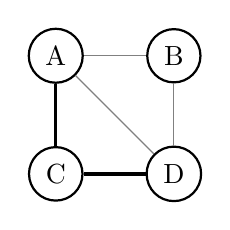
\begin{tikzpicture}[every node/.style={circle,thick,draw}]
    \node (A) at (0, 0) {A};
    \node (B) at (1.5, 0) {B};
    \node (C) at (0, -1.5) {C};
    \node (D) at (1.5, -1.5) {D};

    \path[-] (A) edge[draw=gray,thin] (B);
    \path[-] (A) edge[draw=black,very thick] (C);
    \path[-] (B) edge[draw=gray,thin] (D);
    \path[-] (C) edge[draw=black,very thick] (D);
    \path[-] (A) edge[draw=gray,thin] (D);
  \end{tikzpicture}
  \quad
  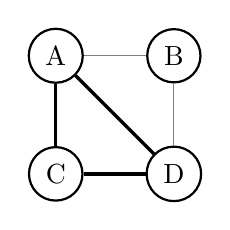
\begin{tikzpicture}[every node/.style={circle,thick,draw}]
    \node (A) at (0, 0) {A};
    \node (B) at (1.5, 0) {B};
    \node (C) at (0, -1.5) {C};
    \node (D) at (1.5, -1.5) {D};

    \path[-] (A) edge[draw=gray,thin] (B);
    \path[-] (A) edge[draw=black,very thick] (C);
    \path[-] (B) edge[draw=gray,thin] (D);
    \path[-] (C) edge[draw=black,very thick] (D);
    \path[-] (A) edge[draw=black,very thick] (D);
  \end{tikzpicture}
  \quad
  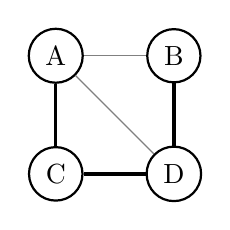
\begin{tikzpicture}[every node/.style={circle,thick,draw}]
    \node (A) at (0, 0) {A};
    \node (B) at (1.5, 0) {B};
    \node (C) at (0, -1.5) {C};
    \node (D) at (1.5, -1.5) {D};

    \path[-] (A) edge[draw=gray,thin] (B);
    \path[-] (A) edge[draw=black,very thick] (C);
    \path[-] (B) edge[draw=black,very thick] (D);
    \path[-] (C) edge[draw=black,very thick] (D);
    \path[-] (A) edge[draw=gray,thin] (D);
  \end{tikzpicture}
  \quad
  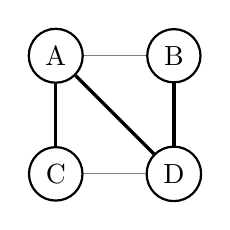
\begin{tikzpicture}[every node/.style={circle,thick,draw}]
    \node (A) at (0, 0) {A};
    \node (B) at (1.5, 0) {B};
    \node (C) at (0, -1.5) {C};
    \node (D) at (1.5, -1.5) {D};

    \path[-] (A) edge[draw=gray,thin] (B);
    \path[-] (A) edge[draw=black,very thick] (C);
    \path[-] (B) edge[draw=black,very thick] (D);
    \path[-] (C) edge[draw=gray,thin] (D);
    \path[-] (A) edge[draw=black,very thick] (D);
  \end{tikzpicture}
  \quad
  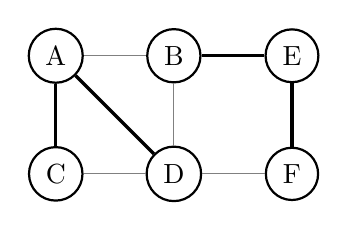
\begin{tikzpicture}[every node/.style={circle,thick,draw}]
    \node (A) at (0, 0) {A};
    \node (B) at (1.5, 0) {B};
    \node (C) at (0, -1.5) {C};
    \node (D) at (1.5, -1.5) {D};
    \node (E) at (3, 0) {E};
    \node (F) at (3, -1.5) {F};

    \path[-] (A) edge[draw=gray,thin] (B);
    \path[-] (A) edge[draw=black,very thick] (C);
    \path[-] (B) edge[draw=gray,thin] (D);
    \path[-] (C) edge[draw=gray,thin] (D);
    \path[-] (A) edge[draw=black,very thick] (D);
    \path[-] (B) edge[draw=black,very thick] (E);
    \path[-] (E) edge[draw=black,very thick] (F);
    \path[-] (D) edge[draw=gray,thin] (F);
  \end{tikzpicture}
\end{center}
The independent sets of a graph are the forests, that is, the subgraphs that do not include cycles.
The dependent sets are the subgraphs that include cycles.

% TODO expand on this definition

\section{Definition of Matroids}

Now that we have some intuition about the concept of ``independence,'' let's give a definition of matroids.\footnote{
  We could define matroids in many ways.
  Matroids are referred to as \emph{cryptomorphic}, which means they have many equivalent but ostensibly unrelated definitions.}
Many mathematical definitions involve placing a set inside of parentheses with other sets or functions that further describe that set.
For example, a graph is given by two sets ${G = (V, E)}$.
A vector space is given by ${(V, k, +, \cdot)}$, where $V$ is a set of vectors, $k$ is a field of scalars, $+$ is an addition of vectors, and $\cdot$ is a multiplication between a scalar and a vector.
A familiar example is ${(\R^3, \R, +, \cdot)}$.
If you have taken CS~$2800$ or other more advanced courses, you will have seen groups, where are often described by writing ${(G, +)}$, where $G$ is a set and $+$ is a binary operation on that set.
Matroids have a similar definition, where we have a set that we write in parentheses together with some other information describing that set.
In this definition the additional information is a collection of subsets.

\begin{defn}[Matroid]
  A \emph{matroid}~$M$ is a pair~$(E, \I)$ consisting of a finite set~$E$ and a collection~$\I$ of subsets of~$E$, called the \emph{independent sets}, satisfying the following properties:
  \begin{enumerate}
    \item The collection is nonempty.
      That is, ${\I \ne \varnothing}$.
    \item All subsets of an independent set are independent.
      That is, if ${A \in \I}$ and ${B \subseteq A}$, then ${B \in \I}$.
    \item If $A$ and $B$ are independent sets and $A$ is larger than $B$, then we can take an element that is in $A$ but not in $B$ and add it to $B$ to construct an independent set.
    That is, if ${A, B \in \I}$ with ${|A| > |B|}$, then there exists ${x \in A \setminus B}$ such that ${B \cup \{x\} \in \I}$.
    This property is knows as the \emph{independent set exchange property}---we can ``exchange'' an element from one set to another.
  \end{enumerate}
  A subset of~$E$ that is not independent is called \emph{dependent}.
\end{defn}

Let's see how this definition fits in with our first two examples.
Recalling that a vector space has a set of vectors~$V$, we form a matroid~$(V, \I)$, where $\I$ is the collection of independent sets of vectors of~$V$.
Recall what we noted previously: given a set of independent vectors, removing vectors still results in an independent set.
And if there are two independent sets of vectors ${A = \{\bv{a}_1, \ldots, \bv{a}_n\}}$ and ${B = \{\bv{b}_1, \ldots, \bv{b}_m\}}$ with ${m < n}$, then clearly $B$ is not a maximal independent set, so we can add more vectors to it while maintaining independence.\footnote{
  See the Steinitz exchange lemma for more details.
}

Next, given an undirected graph ${G = (V, E)}$, we form a matroid~$(E, \I)$ with the ground set given by the graph's edges and the independent sets given by the graph's forests.
Let's verify each part of the definition.
\begin{enumerate}
  \item The empty collection of edges forms a forest vacuously.
  \item If a graph does not form a cycle, then removing edges cannot yield a cycle.
  \item
\end{enumerate}

\section{Kruskal's Algorithm}

Further, note that all spanning trees contain ${|V| - 1}$ edges.

% TODO a few examples/non-examples of spanning trees

% TODO explain spanning tree algorithm
Given a graph

% TODO example graph

Here we are interested in the correctness of this algorithm, and for now we don't consider the implementation details of the algorithm.\footnote{
  If you are interested in the details of an efficient implementation, you can look up the Union-Find data structure.
}
% TODO actually give proof

Matroids are useful beyond just spanning trees.
In general if ${(E, \I)}$ is a matroid, then a greedy algorithm can be used to produce a maximal independent set of minimum weight.
And if ${(E, \I)}$ is not a matroid, then the greedy algorithm fails for some choice of integer weights.
You'll learn more about Greedy Algorithms if you take the undergraduate algorithms course CS~$4820$, and you'll learn more about matroids if you take the graduate algorithms course CS~$6820$ or the combinatorics course sequence~Math~$4410$ and~$4420$.

\end{document}
